\newif\ifshowsolutions
\showsolutionsfalse
\documentclass{article}
\usepackage{listings}
\usepackage{amsmath}
%\usepackage{subfigure}
\usepackage{subfig}
\usepackage{amsthm}
\usepackage{amsmath}
\usepackage{amssymb}
\usepackage{graphicx}
\usepackage{mdwlist}
\usepackage[colorlinks=true]{hyperref}
\usepackage{geometry}
\usepackage{titlesec}
\geometry{margin=1in}
\geometry{headheight=2in}
\geometry{top=2in}
\usepackage{palatino}
\usepackage{mathrsfs}
\usepackage{fancyhdr}
\usepackage{paralist}
\usepackage{todonotes}
\setlength{\marginparwidth}{2.15cm}
\usepackage{tikz}
\usetikzlibrary{positioning,shapes,backgrounds}
\usepackage{float} % Place figures where you ACTUALLY want it
\usepackage{comment} % a hack to toggle sections
\usepackage{ifthen}
\usepackage{mdframed}
\usepackage{verbatim}
\usepackage[strings]{underscore}
\usepackage{listings}
\usepackage{bbm}
\usepackage{poemscol}
\rhead{}
\lhead{}

\fancyfoot[C]{\thepage}
\renewcommand{\baselinestretch}{1.15}

% Shortcuts for commonly used operators
\newcommand{\E}{\mathbb{E}}
\newcommand{\Var}{\operatorname{Var}}
\newcommand{\Cov}{\operatorname{Cov}}
\newcommand{\Bias}{\operatorname{Bias}}
\DeclareMathOperator{\argmin}{arg\,min}
\DeclareMathOperator{\argmax}{arg\,max}

% do not number subsection and below
\setcounter{secnumdepth}{1}

% custom format subsection
\titleformat*{\subsection}{\large\bfseries}

% set up the \question shortcut
\newcounter{question}[section]
\newenvironment{question}[1][]
  {\refstepcounter{question}\par\addvspace{1em}\textbf{Question~\Alph{question}\!
    \ifthenelse{\equal{#1}{}}{}{ [#1 points]}: }}
    {\par\vspace{\baselineskip}}

\newcounter{subquestion}[question]
\newenvironment{subquestion}[1][]
  {\refstepcounter{subquestion}\par\medskip\textbf{\roman{subquestion}.\!
    \ifthenelse{\equal{#1}{}}{}{ [#1 points]:}} }
  {\par\addvspace{\baselineskip}}

\titlespacing\section{0pt}{12pt plus 2pt minus 2pt}{0pt plus 2pt minus 2pt}
\titlespacing\subsection{0pt}{12pt plus 4pt minus 2pt}{0pt plus 2pt minus 2pt}
\titlespacing\subsubsection{0pt}{12pt plus 4pt minus 2pt}{0pt plus 2pt minus 2pt}


\newenvironment{hint}[1][]
  {\begin{em}\textbf{Hint: }}{\end{em}}

\if showsolutions
  \newenvironment{solution}[1][]
    {\par\medskip \begin{mdframed}\textbf{Solution~\Alph{question}#1:} \begin{em}}
    {\end{em}\medskip\end{mdframed}\medskip}
  \newenvironment{subsolution}[1][]
    {\par\medskip \begin{mdframed}\textbf{Solution~\Alph{question}#1.\roman{subquestion}:} \begin{em}}
    {\end{em}\medskip\end{mdframed}\medskip}
\else
  \excludecomment{solution}
  \excludecomment{subsolution}
\fi

\chead{%
  {\vbox{%
      \vspace{2mm}
      \large
      Machine Learning \& Data Mining \hfill
      Caltech CS/CNS/EE 155 \hfill \\[1pt]
      Homework 5\hfill
      February 17th, 2017 \\
      Richard Cheng \hfill
    }
  }
}

\begin{document}
\pagestyle{fancy}

\section*{Tokenizing}

\medskip

The sonnets were initially tokenized by words using the NLTK's function word_tokenizer because word is the smallest entity that we can tokenize in the sonnets such that we can still regenerate sentences with the tokens later. We created two types of data set. First, we consider each line as a sequence, and second, we consider each sonnet as a sequence.

The first change we made after running the learning algorithm was to remove all punctuations. We decided to generate the sentences backward using a seed (i.e. a word) to achieve accurate ending rhythm. Thus, the punctuations were mostly irrelevant because they showed up mostly in the end. In addition, we also find that the model with punctuations generated sentences that sometimes had brackets that did not match or commas that did not make gramatical sense. Therefore, punctuations were removed in our final version.

Furthermore, we counted the bigrams within the sonnets and replaced each pair of consecutive words that showed up frequently in the sonnets as one ``word''. These word pairs were added into the list of all word tokens. In total, 29 pairs of words were added. Each pair appeared in the sonnets at least 15 times. The top five examples were ``my love'', ``thou art'', ``my self'', ``in the '', ``that i'' which appeared 41, 33, 29, 29, and 28 times respectively.

Lastly, we created a rhythm dictionary that was used in poem generation later to create sentences that had the correct rhymes. For the rhythm dictionary, we collected all ending words in each line of the sonnets that rhymed. For example, ``increase'' and ``decrease'' is a pair of words that rhymed. So, they are stored as a tuple in the rhythm dictionary.


\section*{Algorithm}

\medskip

For unsupervised training of our Hidden Markov Model, we used the Baum-Welch algorithm. We used the TA solution from HW \#5 for the implementation. The main three parameters we control were (1) the number of EM iterations, (2) the number of hidden states to use, and (3) whether to train on lines of each poem or the poems themselves  . Regarding (1), we used 1000 iterations, because this was enough iterations to show convergence to a very reasonable precision. Regarding (2) and (3), we trained several different HMMs, each with a different number of hidden states (8, 10, 12, 15, 16, 20, 25, 30). For each choice of hidden states, we also trained on each line of the poem, and on each poem itself. We then visualized the HMMs through both the transition matrix and observation matrix  (discussed in section ***), and examined the generated poems (discussed in section ***) to determine the optimal number of hidden states based on a qualitative analysis of the HMM structure, and whether to train on lines or poems.

~

We eventually chose an HMM with 20 hidden states trained on the individual lines of the poem, based on the underlying structure of the HMM and the qualitative quality of the generated poems. When we assess the underlying structure of the HMM, we refer to meaningful patterns in the transition matrix and observation matrix (also whether states generate words with discernable patterns).

~

When generating our poem, we also needed to keep track of both syllable count. To do this, we used the NLTK CMU dictionary to keep syllable counts.


\medskip

\section*{Poem Generation}

\subsection*{First Bare-Bones Implementation}

For our initial bare-bones implementation, we originally generated poems by the following steps:

~

\begin{enumerate}

\item Pick a uniformly random states to begin at

\item Initialize an empty line and initialize the syllable count of this line to zero.

\item Sample the next state based on the previous state and the transition matrix probabilities.

\item Add a word to the line based on the current state and the observation matrix probabilities

\item Count the number of syllables in the added word and add it to a syllable count

\item Repeat steps 3-5 until we have created a line with at least 10 syllables. Save this line to our poem.

\item Repeat steps 1-6 until we have generated 14 lines for our poem.

\end{enumerate}
~

By following the steps above, we were able to generate 14-line poems with each line containing \textit{at least} 10 syllables. 

\section*{Poem Generation/Additional Goals}

However, we wanted to generate poems with \textit{exactly} 10 syllables. To do this we modified step 6 to get the following algorithm:

\subsection*{Implementation with Syllable Counts (No Rhyme)}

However, we wanted to generate poems with \textit{exactly} 10 syllables. To do this we modified step 6, and get the following algorithm:

\begin{enumerate}

\item Pick a uniformly random states to begin at

\item Initialize an empty line and initialize the syllable count of this line to zero.

\item Sample the next state based on the previous state and the transition matrix probabilities.

\item Add a word to the line based on the current state and the observation matrix probabilities

\item Count the number of syllables in the added word and add it to a syllable count

\item Repeat steps 3-5 until we have created a line with at least 10 syllables. 

\begin{enumerate}

\item If we have exactly 10 syllables. Add the line to the poem

\item If we have \textgreater 10 syllables, remove the last word, go to the previous state and repeat steps 3-5.

\end{enumerate}

\item Repeat steps 1-6 until we have generated 14 lines for our poem.

\end{enumerate}
~

This gave poems with exactly 10 syllables. The tradeoff here was that the last word of the line was often restricted in its number of syllables (i.e. if we had 8 syllables in our line already, we had to pick a last word with less than 3 syllables). Thus the last word was picked from a probability distribution that did not exactly match that given by the bare-bones HMM.

\subsection*{Implementation with Syllable Count and Rhyme}

Finally, we want to implement rhyme. To do this, we had to generate our poems backward using the following algorithm:

~
\begin{enumerate}

\item Create a dictionary of rhyming pairs based on the rhyming pairs in the shakespeare poems we trained on. 

\item For lines 1, 2, 5, 6, 9, 10, 13, randomly choose a word from the rhyming dictionary. For all other lines, choose the rhyming word that goes with the corresponding line (e.g. for line 4, choose the rhyming word from our rhyming dictionary that is paired with the word chosen for line 2). 

\item Sample the state based on calculated probability $P(y \mid x)$ where $y$ represents a hidden state and $x$ represents our observation of the first word. We can calculate $P(y \mid x)$ using the formula $P(y^1 = z \mid x) = \frac{\alpha_z(1) \beta_z(1)}{\sum_{z'} \alpha_{z'} (1) \beta_{z'}(1)}$. We use the \textit{forward, backward} functions we wrote for HW \#5 in order to get $\alpha$ and $\beta$. One we have our chosen first word and have calculated $P(y \mid x)$, we can sample from this distribution to get $y^1$.

\item Add a word to the line based on the current state and the observation matrix probabilities

\item Count the number of syllables in the added word and add it to a syllable count

\item Sample the next state based on the previous state and the transition matrix probabilities.

\item Add a word to the line based on the current state and the observation matrix probabilities

\item Count the number of syllables in the added word and add it to a syllable count

\item Repeat steps 6-8 until we have created a line with at least 10 syllables. 

\begin{enumerate}
\item If we have exactly 10 syllables. Add the line to the poem

\item If we have \textgreater 10 syllables, remove the last word, go to the previous state and repeat steps 6-8

\end{enumerate}

\item Reverse the generated line (because we have generated the line backwards to ensure proper rhyming), and add it to the poem.

\item Repeat steps 2-10 until we have generated 14 lines.

\end{enumerate}
~

\subsection*{Generation Result/Discussion}

Using this algorithm, we were able to successfully automatically generate poems using an HMM trained on several shakespeare poems that obeyed the syllable count and rhyming pattern of a shakespearean sonnet. However, by implementing rhyme in the above fashion, we had to restrict the choice of first word in every line to one from our rhyming dictionary. Thus the structure of our generation algorithm using HMM was different. In our first step, rather than transitioning to an initial state (based on A) and generating a word (based on O), we had to first choose the word, and then sample the most likely state.

Generating the poems backward in this fashion had the effect:

\begin{enumerate}

\item Because we were considering transitions backward (to the previous word in the line), the state transition matrix became less intuitive to follow since reading sentences backwards is less natural to humans and may show different structure.

\item Sometimes the first word of each line (the last generated word of the line since we generated backwards) often did not fit as a first word. 

\item Our first word of each line was limited to our rhyming dictionary. Furthermore, we had to calculate $P(y \mid x)$ in order to get the first state from the first word, 

\end{enumerate}

Below is one of the poems we generated with the proper rhyming scheme and syllable count (chosen for Piazza submission):

\begin{poem}
\begin{stanza}
Love my self alteration side granting \verseline
Plague for and bright oaths but sit faces moan \verseline
Sky grow'st best wilt or not to on wanting \verseline
Up turns abide votary shall upon
\end{stanza}
\begin{stanza}
Not bide canst the that which to oppressed \verseline
Am too black try is fair am be increase \verseline
Usurer in chest state party age rest \verseline
Change of in not to knows my muse decease 
\end{stanza}
\begin{stanza}
Can canker be war him forth him power \verseline
Days loss is ward clock dead eloquence pride \verseline
I still verse with abide play'st call flower \verseline
Again cruel told kindness odour one side  \end{stanza}
\begin{stanza}
Than to that i west slow and sounds a reap \verseline
All friend great poor tear that all that i leap \end{stanza}
\end{poem}


The poems we generated had some structure and some grammatically sensical lines. However, it suffered from a few shortcomings discussed below.

\begin{enumerate}

\item By nature of generation with HMMs, words can only have direct relation with the previous word. Therefore it becomes likely for sentences to wander, and difficult to string together more than a few words for a single coherent idea. Thus, in our poems, seldom are there long strings of words forming a single coherent idea. 

\item Because we trained our HMM on individual lines, the generated poems had no theme (beyond the coincidental). Thus each line often showed little thematic correlation to adjacent lines.

\item Some words or pairs of words were extremely frequent in the poems, and the prominence of common words like 'the', 'be', and 'he' often threw off the structure of sentences. Interestingly, the word 'love' shows up in Shakespeare's poems frequently, so this word also showed up in our poems very frequently.

\end{enumerate}


\medskip

\section*{Visualization and Interpretation}

The top 10 words that associate with the hidden state are given in Table \ref{tab:top-10-words} (the numbers below the words denote the probability). The number in bracket is the total number of top words to form approximately 0.5 probability. Hidden state 11 and 12 have probabilities that are more diffused and they includes more words that are nouns, adverbs or adjectives. Hidden state 1, 8, 9, and 18 have a more concentrated probabilities, and they tend to be words that are used to connect phrases like particles, conjunctions, and pronouns. Hidden state 10 includes the 5 ``wh'' words for questions. 

Figure \ref{fig:observation-matrix} shows the observation matrix in which each row is normalized to 0 and 1 for clearer color constrast. Each column represents a token and the columns are sorted by the frequency of the tokens. The top plot shows all tokens, and the bottom plot shows the first 100 tokens. From the plots, we can see that the most common words in general have a higher probability than the less common words. Words like ``and'' which are very frequently used (473 times) in the sonnets show up in a few hidden states with high probability.

If we also consider the transition matrix (Figure \ref{fig:state-transition}), we can observe some interesting state transitions that makes gramatical sense. For example, hidden state 11 is most likely to transition to hidden state 19 with probability 0.9330. Combinations of the top 4 words ``of'', ``in'', ``to'', and ``not'' in hidden state 19 with most of the top 10 words in hidden state 11 (e.g. love, i, one, hath, beauty, this, and most) seem to make gramatical sense. Another example is hidden state 1 is most likely to transition to hidden state 12 with probability 0.9836. Combinations of the top words ``is'' and ``time'' in hidden state 12 with ``the'', ``my'', ``a'', ``so'', ``such'', ``their'', ``his'', and ``of the'' in hidden state 1 also make gramatical sense.


\begin{table}[h!]
	\centering
	\caption{Top 10 words for hidden states and the probability. The number in bracket is the total number of top words to form approximately 0.5 probability.}\label{tab:top-10-words}
	\begin{tabular}{c||l|l|l|l|l|l|l|l|l|l}
		\hline
		State & \multicolumn{10}{c}{Top 10 Words}\\ \hline
		0 & in & the & by & own & my & with & make & to & show & your \\
		(26) & 0.1054 & 0.0399 & 0.0352 & 0.0300 & 0.0250 & 0.0244 & 0.0230 & 0.0230 & 0.0149 & 0.0140 \\ \hline
		1 & the & my & a & so & such & their & his & of the & well & thine \\
		(9) & 0.2325 & 0.0604 & 0.0481 & 0.0337 & 0.0319 & 0.0283 & 0.0251 & 0.0204 & 0.0164 & 0.0158 \\ \hline
		2 & so & not & and & of & a & thy & me & self & youth & thee \\
		(50) & 0.0364 & 0.0248 & 0.0247 & 0.0234 & 0.0223 & 0.0203 & 0.0195 & 0.0169 & 0.0143 & 0.0140 \\ \hline
		3 & all & to & that & for & the & from & with & you & he & yet \\
		(23) & 0.0454 & 0.0417 & 0.0413 & 0.0400 & 0.0313 & 0.0305 & 0.0236 & 0.0221 & 0.0192 & 0.0187 \\ \hline
		4 & be & but & more & are & you & which & is & her & so & i am \\
		(30) & 0.0444 & 0.0407 & 0.0402 & 0.0401 & 0.0332 & 0.0262 & 0.0257 & 0.0205 & 0.0179 & 0.0177 \\ \hline
		5 & and & that & for & so & no & now & then & eyes & to me & when i \\
		(35) & 0.0985 & 0.0387 & 0.0361 & 0.0311 & 0.0217 & 0.0210 & 0.0152 & 0.0150 & 0.0148 & 0.0128 \\ \hline
		6 & my & it & they & me & i & but & those & this & her & is \\
		(15) & 0.0993 & 0.0854 & 0.0403 & 0.0371 & 0.0271 & 0.0259 & 0.0257 & 0.0228 & 0.0226 & 0.0205 \\ \hline
		7 & to & thy & your & my & not & or & the & dost & on & as \\
		(21) & 0.0702 & 0.0565 & 0.0442 & 0.0384 & 0.0333 & 0.0318 & 0.0217 & 0.0215 & 0.0201 & 0.0167 \\ \hline
		8 & and & which & so & who & therefore & if & even & not & or & for \\
		(2) & 0.3856 & 0.0657 & 0.0509 & 0.0439 & 0.0202 & 0.0189 & 0.0136 & 0.0134 & 0.0112 & 0.0106 \\ \hline
		9 & and & that & as & but & when & how & which & since & for & can \\
		(3) & 0.2786 & 0.0876 & 0.0825 & 0.0707 & 0.0523 & 0.0423 & 0.0287 & 0.0221 & 0.0193 & 0.0151 \\ \hline
		10 & if & what & that & nor & when & where & the & let & why & how \\
		(10) & 0.0723 & 0.0719 & 0.0719 & 0.0502 & 0.0492 & 0.0400 & 0.0380 & 0.0336 & 0.0311 & 0.0221 \\ \hline
		11 & love & i & one & hath & beauty & this & most & in the & will & part \\
		(61) & 0.0354 & 0.0265 & 0.0209 & 0.0208 & 0.0200 & 0.0185 & 0.0178 & 0.0177 & 0.0175 & 0.0149 \\ \hline
		12 & is & time & eyes & do & should & a & sun & summer & age & best \\
		(81) & 0.0305 & 0.0235 & 0.0183 & 0.0143 & 0.0126 & 0.0116 & 0.0105 & 0.0101 & 0.0100 & 0.0095 \\ \hline
		13 & i & that & with & not & my & do & did & she & see & is \\
		(31) & 0.0914 & 0.0403 & 0.0359 & 0.0352 & 0.0342 & 0.0220 & 0.0197 & 0.0193 & 0.0180 & 0.0168 \\ \hline
		14 & thy & a & his & in & you & your & sweet & have & the & with \\
		(18) & 0.0958 & 0.0783 & 0.0379 & 0.0368 & 0.0294 & 0.0269 & 0.0267 & 0.0252 & 0.0237 & 0.0196 \\ \hline
		15 & thou & of & is & in & all & being & and & were & from & day \\
		(31) & 0.1502 & 0.0474 & 0.0367 & 0.0202 & 0.0170 & 0.0162 & 0.0136 & 0.0133 & 0.0126 & 0.0114 \\ \hline
		16 & to & i & doth & mine & and & than & shall & as & by & thine \\
		(19) & 0.1011 & 0.0712 & 0.0368 & 0.0312 & 0.0304 & 0.0244 & 0.0223 & 0.0199 & 0.0197 & 0.0194 \\ \hline
		17 & thee & with & me & be & love & is & their & all & this & heart \\
		(28) & 0.0661 & 0.0605 & 0.0547 & 0.0405 & 0.0358 & 0.0269 & 0.0249 & 0.0176 & 0.0168 & 0.0155 \\ \hline
		18 & o & but & for & or & then & yet & against & save & to & when \\
		(3) & 0.1761 & 0.1683 & 0.1355 & 0.0924 & 0.0595 & 0.0321 & 0.0303 & 0.0241 & 0.0198 & 0.0169 \\ \hline
		19 & of & in & to & not & i & doth & and & will & do & of thy \\
		(14) & 0.1831 & 0.0562 & 0.0431 & 0.0380 & 0.0269 & 0.0249 & 0.0205 & 0.0200 & 0.0166 & 0.0150 \\ \hline
	\end{tabular}
\end{table}

\begin{figure}[h!]
	\centering
	\subfloat{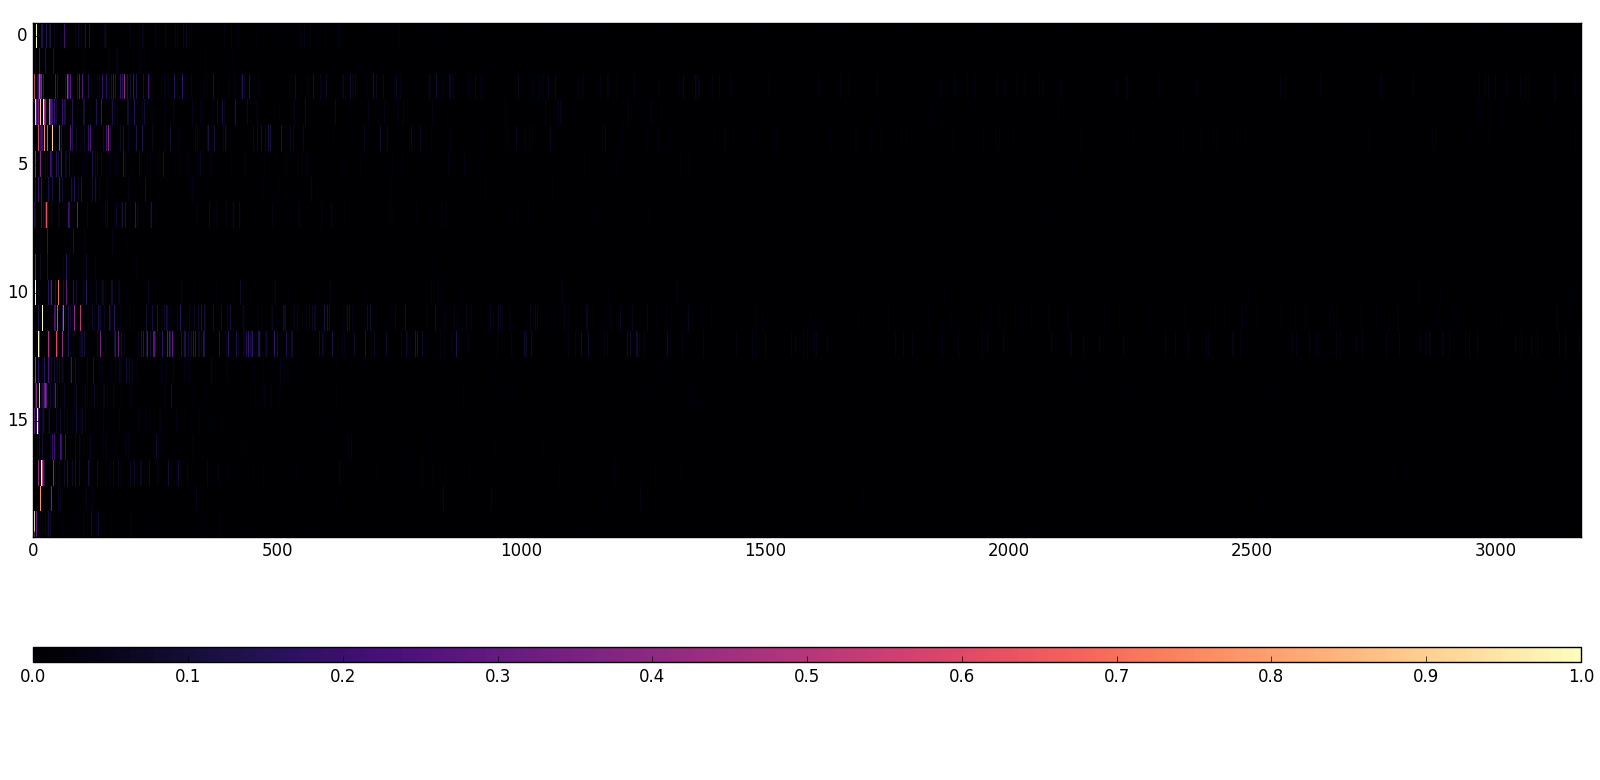
\includegraphics[width=\textwidth, clip=true, trim=0cm 2cm 0cm 0cm]{observation_matrix_normalized}} \\
	\subfloat{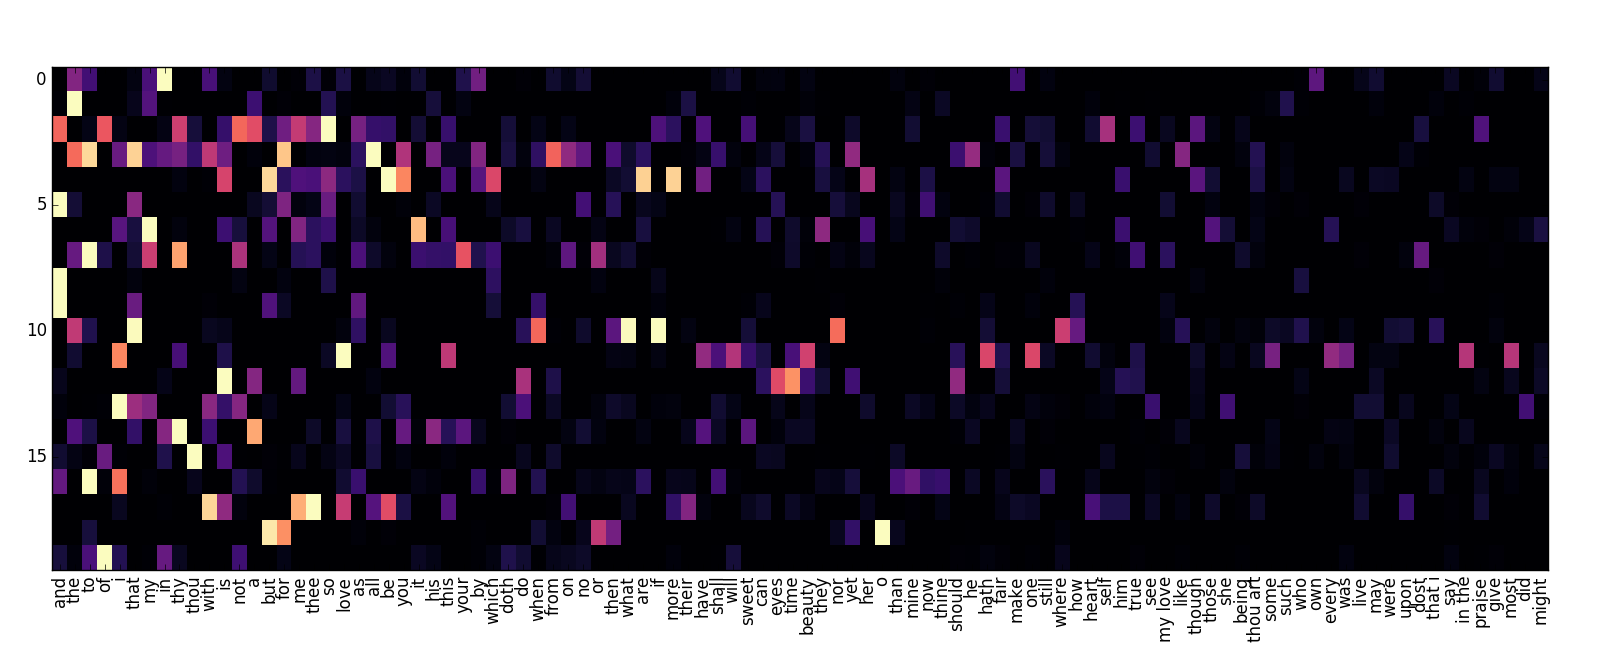
\includegraphics[width=\textwidth, clip=true, trim=0.5cm 0cm 1cm 0cm]{observation_matrix_normalized_zoom}} 
	\caption{Normalized observation matrix. The top plot shows all tokens, and the bottom plot zooms into the first 100 tokens.}\label{fig:observation-matrix}
\end{figure}

\begin{figure}[h!]
	\centering
	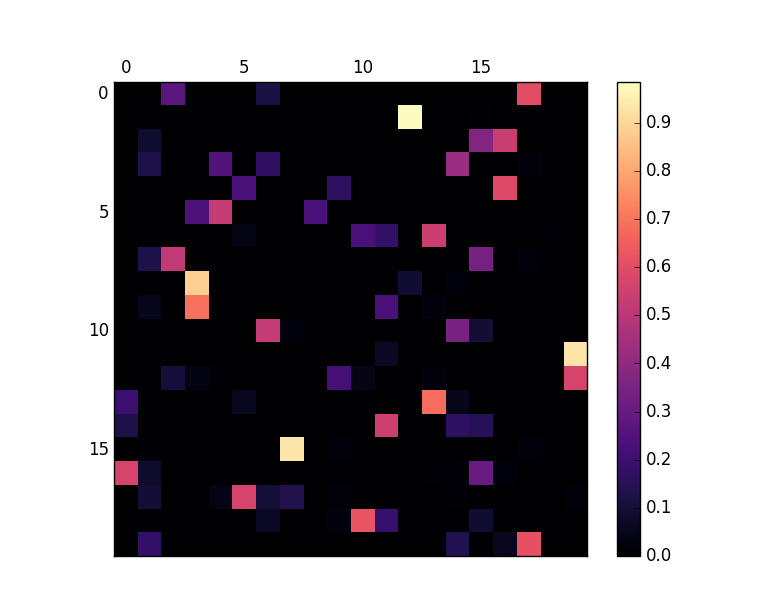
\includegraphics[width=0.65\textwidth, clip=true, trim=1cm 1cm 1cm 1cm]{transition_matrix}
	\caption{State transition matrix}\label{fig:state-transition}
\end{figure}



\end{document}
